\section{Methoden}\label{sec:event-storming}
In diesem Unterkapitel werden die grundlegenden Prinzipien und Ziele des \ac{DDD} erläutert, welche Vaughn Vernon in seinem Buch
\textit{Domain-Driven Design Distilled} definiert hat\cite*{dddd}.
Nachdem diese Grundlage vorhanden ist, wird darauf aufbauend erklärt, welche Symbiose aus dem \ac{DDD} und dem \ac{ES} entsteht und wie
dies zu einer Softwareentwicklung beiträgt.
Abschließend werden die neuen Ansätze zum~\ac{ES}, welche im Kontext dieser Arbeit vorgenommen wurden, erklärt.

\subsection{Domain-Driven Design}\label{subsec:domain-driven-design}
Das \ac*{DDD} ist nicht nur für die erste Phase der Softwareentwicklung praktisch, sondern ebenso für das Umstrukturieren bestehender Projekte.
Ein grundlegendes Ziel des \ac{DDD} ist es ein Projekt in sogenannte \textit{Bounded Contexts} zu unterteilen und damit zu umgehen, dass
die Anwendung aus einem riesigen aufgeblähten Modell besteht.
Um dieses Ziel zu erreichen, ist es wichtig in Gesprächen mit Domänenexperten die wichtigsten Punkte eines \textit{Bounded Context} zu evaluieren.
Domänenexperten können in jedem Bereich eines Unternehmens gefunden werden.
Es ist nötig ein möglichst breites Spektrum an Personen zu haben, um den gesamten zu entwickelnden Prozess zu verstehen und für die Entwickler verständlich zu machen.
Dabei ist es wichtig, dass alle Personen, welche am Prozess des \ac{DDD} teilnehmen, eine einheitliche Sprache entwickeln.
Diese einheitliche Sprache beschreibt Vernon als~\textit{Ubiquitous Language}\footnote{im Deutschen ``allgegenwärtige Sprache''}\cite*{dddd}.
Diese Sprache zu entwickeln, ist eine fortlaufende Aufgabe für die im Projekt angesiedelten Personen.
Initial ist es wichtig, dass zwischen den verschiedenen Domänenexperten und den Entwicklern diese allgegenwärtige Sprache entsteht, welche
nicht nur das Verständnis zwischen den beiden Parteien verbessern, sondern auch mit in das Modell einfließen soll.

\subsection{Event Storming}\label{subsec:allgemein}
Vernon selbst nennt Event Storming als mögliche Methode, um eine~\textit{Ubiquitous Language}\cite*{dddd} zu entwickeln.
Event Storming wurde von Alberto Brandolini entwickelt und resultiert aus mangelnder Zeit während der Nutzung von~\textit{event-driven modeling}.
\textit{Event-driven modeling} basiert ebenfalls auf Konversationen und konkreten Szenarien, allerdings mit der Verwendung von UML-Diagrammen zur Datenmodellierung.
Dies hatte zur Konsequenz, dass in Gesprächen zur Anforderungsanalyse ab einem bestimmten Punkt nur noch die Entwickler daran teilnahmen.
Brandolini verwarf UML-Diagramme, verwendete stattdessen Haftnotizen und legte damit den Grundbaustein für das~\ac{ES}\cite*{dddd}.

In seinem Buch ``Introducing EventStorming'' beschreibt Brandolini mehrere \ac{ES}-Workshops und wie diese durchgeführt wurden\cite*{introES}.
Hierbei stellt sich heraus, dass Event Storming kein starres Konstrukt aus Abläufen ist, sondern je nach Kontext angepasst werden kann.
Dennoch gibt es Ähnlichkeiten, welche eine solide Grundlage für einen \ac{ES}-Workshop bieten\cite*{introES}.
Neben einem grenzenlosen Platz zum Modellieren benötigt es genügend Marker und Haftnotizen in verschiedenen Formen und Farben.
Die teilnehmenden Domänenexperten benötigen eine kollaborative Einstellung zur Modellierung, ein offenes Miteinander ungeachtet ihrer Stellung.
Zudem sollte es zu Beginn eines Projektes und dem damit einhergehenden \ac{ES}-Workshop keine Grenzen zu dem Thema oder der Anwendung welche modelliert werden soll geben.
Dadurch sollen weitere Probleme gelöst oder Fragen beantwortet werden.
Ein Event Storming beginnt immer mit dem Erstellen von Domain Events und dem Platzieren dieser anhand eines Zeitstrahles.
Zudem müssen alle Beteiligten am fortlaufenden Verfeinern eines Modells interessiert sein, da ein \ac{ES}-Workshop zum Lernen und Verbessern
von Anwendungen gedacht ist.
Ein \ac{ES}-Board nach einem solchen Workshop ist in Abbildung~\ref{fig:rlBoard} dargestellt\cite*{esBoard}.

\begin{figure}[ht]
    \centering
    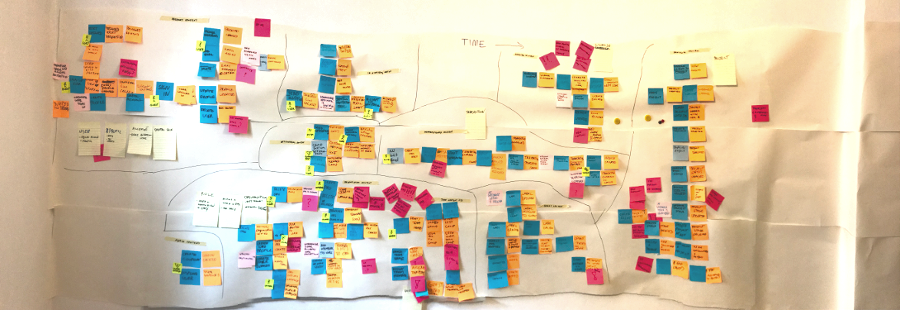
\includegraphics[width=0.75\textwidth]{images/2.1/event-storming}
    \caption{Event-Storming-Board}
    \label{fig:rlBoard}
\end{figure}

Nachdem initial Domain Events beim \ac{ES} erstellt wurden, soll jedem ein Command vorausgesetzt werden.
Ein Command fungiert hierbei als die Aktion, welche das Event ausgelöst hat.
Dies können Aktionen eines Nutzers oder eines externen Systems sein.
Während eines Workshops können sogenannte \textit{Hotspots} in Gesprächen entdeckt werden.
Dabei kann es sich um Probleme, aber auch um Fragen bezüglich des Ablaufs handeln, welche wichtig für die spätere Anwendung werden.

Wie auch das~\ac{DDD} kann Event Storming jederzeit während des Entwicklungsprozesses verwendet werden.
Für die verschiedenen Anwendungsbereiche hat Brandolini mehrere Typen des Event Stormings definiert\cite*{introES}.
Hierbei bleibt die Methodik an sich die gleiche, allerdings wird das Ziel genauer definiert.\newline
\textbf{Big Picture EventStorming} wird während einem Kick-off-Meeting eingesetzt, damit alle Teilnehmer den Inhalt und den Bereich der zu erstellenden Anwendung kennenlernen.
Hierzu ist es nötig, dass alle Interessengruppen vertreten sind, welche innerhalb des Unternehmens existieren und ebenfalls eine Entscheidungsgewalt innehaben.\newline
\textbf{Design Level EventStorming} findet auf einer tieferen Ebene einen Einsatz.
Dabei handelt es sich um das Erstellen möglicher Implementierungen, zum Beispiel, ob Event Sourcing oder andere Techniken aus dem~\ac{DDD} verwendet werden sollen.
Es werden somit Entscheidungen getroffen, welcher in erster Linie die Entwickler betrifft und von diesen am besten zu bewerten ist.\newline
\textbf{Value-Driven EventStorming} bietet einen Einstieg in die Wertstromanalyse (englisch: value-stream mapping).
Anhand einer solchen Analyse ist es möglich den Erhalt von Informationen und der Verarbeitung dieser darzustellen und Probleme zu erkennen.\newline
\textbf{UX-Driven EventStorming} konzentriert sich auf das Erlebnis eines Nutzers/Kunden bei der Benutzung der Anwendung.
Hierbei wird neben der Nutzerfreundlichkeit auch die fehlerfreie Ausführung abgebildet und überprüft.\newline
\textbf{EventStorming as a Retrospective} konzentriert sich darauf einen Ablauf über Domain Events zu definieren und nach
Erweiterungsmöglichkeiten zu suchen, welche Vorteile für die Anwendung bereitstellen können.\newline
\textbf{EventStorming as a Learning Tool} zeigt auch die weiteren Lernchancen innerhalb eines Unternehmens.
Mittels Event Storming ist es somit auch möglich neue Angestellte möglichst schnell auf den aktuellen Stand zu bringen.
Diese Art von Lernchancen ist ebenfalls im~\textbf{Big Picture EventStorming} enthalten.

\subsection{Erweiterung}\label{subsec:erweiterung}
Im Rahmen dieser Arbeit werden verschiedene Bereiche des Event Stormings vertieft.
Zum einen ist dies das Verbildlichen von Arbeitsabläufen, im Folgenden ``Workflows'' genannt.
Ein komplexeres System soll durch die Beschreibung von mehreren Workflows genauer betrachtet werden.
Dies orientiert sich stark an dem zuvor beschriebenen~\textbf{Big Picture EventStorming}, da ein großer Prozess in mehrere kleine
Prozesse aufgeteilt wird und daraus ein \ac{ES}-Board entsteht, welches weiterhin den großen Prozess zeigt.

Zum anderen wurde bei der Entwicklung der Anwendung darauf Wert gelegt, die Generierung von Mockups zu ermöglichen.
Durch diese Möglichkeit ist das zuvor beschriebene \textbf{UX-Driven EventStorming} ein weiterer Typ des Event Stormings, welcher hierbei Verwendung findet.
Die Generierung von Mockups und rudimentären \textit{Clickdummys} soll es ermöglichen, während einem Event Storming genauer auf Oberflächen eingehen zu können
und daraus verschiedene Wege darzustellen, in welcher eine Anwendung genutzt werden kann.

Auf die Generierungsmöglichkeiten von Mockups und deren weitere Funktionen im Web-Editor wird in Kapitel~\ref{ch:implementierung} genauer eingegangen.

